\documentclass{article}

\usepackage[letterpaper]{geometry}
\usepackage{amsmath}
\usepackage{amsfonts}
\usepackage{amssymb}
\usepackage{graphicx}

\title{4123 HW 5}
\author{Duncan Wilkie}
\date{18 November 2021}

\begin{document}

\maketitle

\section{}
The charged particle Lagrangian is, in terms of the generalized coordinate $r$ and potentials $\vec{A}$ and $V$,
\[L=\frac{1}{2}m\dot{q_i}^2+Q\dot{q_i}A_i-QV\]
The generalized momentum is
\[p_i=\frac{\partial L}{\partial\dot{q_i}}=m\dot{q_i}+QA_i\Leftrightarrow \dot{q_i}={\frac{p_i-QA_i}{m}}\]
Plugging this in to the definition of the Hamiltonian, we obtain
\[\mathcal{H}(p_i,q_i)=p_i\dot{q_i}-L=p_i{\frac{p_i-QA_i}{m}}- {\frac{(p_i-QA_i)^2}{2m}}-QA_i{\frac{p_i-QA_i}{m}}+QV\]
\[=(p_i-QA_i)\frac{p_i-QA_i}{m}-\frac{(p_i-QA_i)^2}{2m}+QV\]
\[=\frac{(p_i-QA_i)^2}{2m}+QV\]
From this, we obtain two Hamilton's equations of motion:
\[\dot{q_i}=\frac{\partial\mathcal{H}}{\partial p_i}=\frac{p_i-QA_i}{m}\]
\[\dot{p_i}=-\frac{\partial \mathcal{H}}{\partial q_i}=0\]
These ought to imply the Lorentz force law.

\section{}
The Lagrangian for such a system is
\[L=\frac{1}{2}m\dot{q}^2-mgq\]
The generalized momentum is
\[p=\frac{\partial L}{\partial \dot{q}}=m\dot{q}\Leftrightarrow \dot{q}=\frac{p}{m}\]
Plugging this in to the definition of the Hamiltonian,
\[\mathcal{H}(p,q)=p\dot{q}-L=\frac{p^2}{2m}+mgq\]
The corresponding Hamilton's equations are
\[\dot{q}=\frac{\partial \mathcal{H}}{\partial p}=\frac{p}{m}\]
\[\dot{p}=-\frac{\partial\mathcal{H}}{\partial q}=-mg\]
Integrating the second equation with respect to $t$,
\[p=-mgt+p_0\Rightarrow \dot{q}=-gt+\frac{p_0}{m}\Rightarrow q=-\frac{gt^2}{2}+\frac{p_0}{m}+q_0\]
The phase-space vector of the system is then
\[\vec{z}=\left(p_0-mgt, q_0+\frac{p_0}{m}-\frac{1}{2}gt^2\right)\]
If we take $q_0=0$ and $p_0$ negative, consistent with throwing an object upward from the ground, the plot of the parametric curve in phase space is just a parabola, since the first component being linear is just a rescaling of the horizontal axis (i.e. this is equivalent to the second component under a coordinate transformation $t\mapsto (p_0-q)/mg$). A plot appears below with some test values:

\[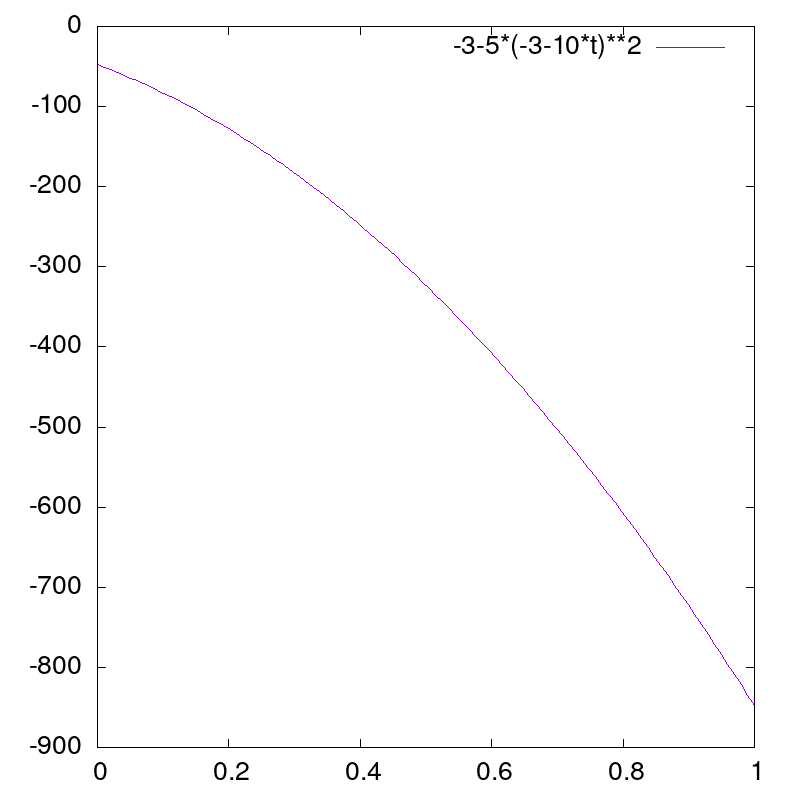
\includegraphics[scale=0.4]{phaseplot.png}\]

\section{}
In cylindrical coordinates, the Lagrangian of a free particle is
\[L=\frac{1}{2}m(\dot{r}^2+r^2\dot{\theta}^2+\dot{z}^2)\]
The generalized momenta are
\[p_r=\frac{\partial L}{\partial \dot{r}}=m\dot{r}\]
\[p_\theta=\frac{\partial L}{\partial \dot{\theta}}=mr^2\dot{\theta}\]
\[p_z=\frac{\partial L}{\partial\dot{z}}=m\dot{z}\]
Therefore, we may write the Lagrangian as
\[L=\frac{1}{2m}\left[ p_r^2+\left( \frac{p_\theta}{r} \right)^2+p_z^2 \right]\]
The Hamiltonian is by definition
\[\mathcal{H}=\sum_ip_i\dot{q}_i-L=\frac{p_r^2}{m}+\frac{p_\theta^2}{mr^2}+\frac{p_z^2}{m}-\frac{p_r^2}{2m}-\frac{p_\theta^2}{2mr^2}-\frac{p_z^2}{2m}\]
\[=\frac{1}{2m}\left( p_r^2+\frac{p_\theta^2}{r^2}+{p_z^2} \right)\]
In spherical coordinates, the Lagrangian of a free particle is
\[L=\frac{1}{2}m(\dot{r}^2+r^2\dot{\theta}^2+r^2\sin^2\theta\dot{\varphi}^2)\]
The generalized momenta are
\[p_r=\frac{\partial L}{\partial\dot{r} }=m\dot{r}\]
\[p_\theta=\frac{\partial L}{\partial\dot{\theta}}=mr^2\dot{\theta}\]
\[p_\varphi=\frac{\partial L}{\partial\dot{\varphi}}=mr^2\sin^2\theta\dot{\varphi}\]
Therefore, we may write the Lagrangian as
\[L=\frac{1}{2m}\left[  p_r^2+\left( \frac{p_\theta}{r} \right)^2+\left( \frac{p_\varphi}{r\sin\theta} \right)^2 \right]\]
The Hamiltonian is by definition
\[\mathcal{H}=\sum_ip_i\dot{q}_i-L=\frac{p_r^2}{m}+\frac{p_\theta^2}{mr^2}+\frac{p_\varphi^2}{mr^2\sin^2\theta}-\frac{p_r^2}{2m}-\frac{p_\theta^2}{2mr^2}-\frac{p_\varphi^2}{2mr^2\sin^2\theta}\]
\[=\frac{p_r^2}{2m}+\frac{p_\theta^2}{2mr^2}+\frac{p_\varphi^2}{2mr^2\sin^2\theta}\]

This suggests a general method for converting Hamiltonians between (some subset of) coordinate systems.

\section{}
We consider the problem in spherical coordinates. If $F=-\nabla U=-k\vec{r}$, we have a potential \[U=\frac{k}{2}\left(x^2+y^2+z^2\right)=\frac{k}{2}\left(r^2\cos^2\theta+r^2\sin^2\theta+z^2\right)=\frac{k}{2}\left( r^2+z^2 \right)\]
The Lagrangian, including the constraint $r=R$ and its Lagrange multiplier, is
\[L=\frac{1}{2}m(\dot{r}^2+r^2\dot{\theta}^2+\dot{z}^2)-\frac{k}{2}\left( r^2+z^2 \right)\]
The generalized momenta are
\[p_r=\frac{\partial L}{\partial \dot{r}}=m\dot{r}\]
\[p_\theta=\frac{\partial L}{\partial\dot{\theta}}=mr^2\dot{\theta}\]
\[p_z=\frac{\partial L}{\partial\dot{z}}=m\dot{z}\]
The Hamiltonian is, in terms of these quantities,
\[\mathcal{H}=\sum_ip_i\dot{q}_i-L=\frac{p_r^2}{m}+\frac{p_\theta^2}{mr^2}+\frac{p_z^2}{m}+\frac{k}{2}\left( r^2+z^2 \right)-\frac{1}{2}m\left( \frac{p_r^2}{m^2}+r^2\frac{p_\theta^2}{m^2r^4}+\frac{p_z^2}{m^2} \right)\]
Since $r=R$, this becomes
\[\mathcal{H}=\frac{p_r^2}{2m}+\frac{p_\theta^2}{2mR^2}+\frac{p_z^2}{2m}+\frac{k}{2}\left( R^2+z^2 \right)\]
The Hamilton's equations are
\[\dot{r}=\frac{\partial \mathcal{H}}{\partial {p_r}}=\frac{p_r}{m}\]
\[\dot{\theta}=\frac{\partial\mathcal{H}}{\partial{p_\theta}}=\frac{p_\theta}{mR^2}\]
\[\dot{z}=\frac{\partial\mathcal{H}}{\partial{p_z}}=\frac{p_z}{m}\]
\[\dot{p_r}=-\frac{\partial\mathcal{H}}{\partial r}=0\]
\[\dot{p_\theta}=-\frac{\partial\mathcal{H}}{\partial \theta}=0\]
\[\dot{p_z}=-\frac{\partial\mathcal{H}}{\partial z}=-kz\]
From this, $\dot{r}$ and $\dot{\theta}$ are constant (the former being actually zero from the constraint), and the interesting equations of motion are
\[\dot{z}=\frac{p_z}{m}\]
\[\dot{p_z}=-kz\]

\end{document}
%%% Local Variables:
%%% mode: latex
%%% TeX-master: t
%%% End:
